\chapter{Uso de inteligencia artificial}
\label{anx:uso-ia}

Este anexo declara el uso de inteligencia artificial en el trabajo, que se ha hecho con supervisión humana (\textit{human in the loop}). El autor plantea cada tarea como un problema y diseña los agentes y flujos de trabajo que la resuelven, con herramientas para comprobar lo que producen. El alcance y las tres fuentes de inclusión de las APIs vienen del encargo del trabajo, y el autor fija las preguntas de investigación y el índice.
Después revisa los datos que los agentes no pueden cerrar con una fuente y las dudas de modelado en las que los agentes no se ponen de acuerdo, y los da por buenos o los corrige. El resto de las tareas lo ejecuta Claude, el asistente de Anthropic, dentro de las reglas que fija el autor.

La Figura~\ref{fig:uso-ia:agentes} recoge cómo se reparte el trabajo.
La sesión principal de Claude, la conversación en la que trabaja el autor, es el coordinador: reparte las tareas entre agentes y, cuando sus propuestas no coinciden, convoca el desempate.
Unos agentes construyen cada Datasheet.
Otro agente, distinto, la verifica: recibe solo la Datasheet terminada, vuelve a abrir cada URL citada y contrasta dato a dato.
La Datasheet pasa además tres comprobaciones automáticas: el validador de formato, la verificación de que cada cita sigue en la copia archivada de su página, cuando la hay, y una ejecución sobre PRIME4API que confirma que el motor carga la Datasheet.

La Datasheet de Postmark, la del piloto, es anterior a este reparto y se cerró sin informe de verificador.
Las otras siete lo tienen.
Las páginas que cita no se archivaron, así que la comprobación de citas no tiene con qué contrastarlas.
La de Postmark sí pasó por el validador de formato y por PRIME4API (Tabla~\ref{tab:verificacion}).

El libro de criterios es el fichero de reglas de modelado que se aplica a todas las Datasheets.
Una de sus reglas dice, por ejemplo, que la política de retención de datos no es una cuota.
Las dudas que ese libro no resuelve las deliberan cinco agentes en paralelo, y si no coinciden, un sexto agente las examina por separado y propone el veredicto, que entra en el libro como regla nueva.
Si tampoco el sexto desempata, la duda pasa al autor.

La comparación entre versiones de los términos de consumo de cada proveedor, que detecta qué cambió entre dos capturas fechadas, la hizo Claude en sesiones independientes.
Es la parte menos formalizada, y por eso se dibuja con borde discontinuo.
Ni las instrucciones que recibió ni los programas que extraen el texto de las versiones archivadas en la Wayback Machine, el archivo de páginas web de Internet Archive, están en el repositorio ni empaquetados como \textit{skill}.
Solo se conservan sus resultados, las tablas de versiones de cada proveedor.
La captura de la versión vigente de cada página sí está versionada, porque la hace la \textit{skill} de recogida descrita en la Sección~\ref{sec:propuesta:ciclo}.

\begin{figure}[H]
\centering
\begingroup\hyphenpenalty=10000\relax
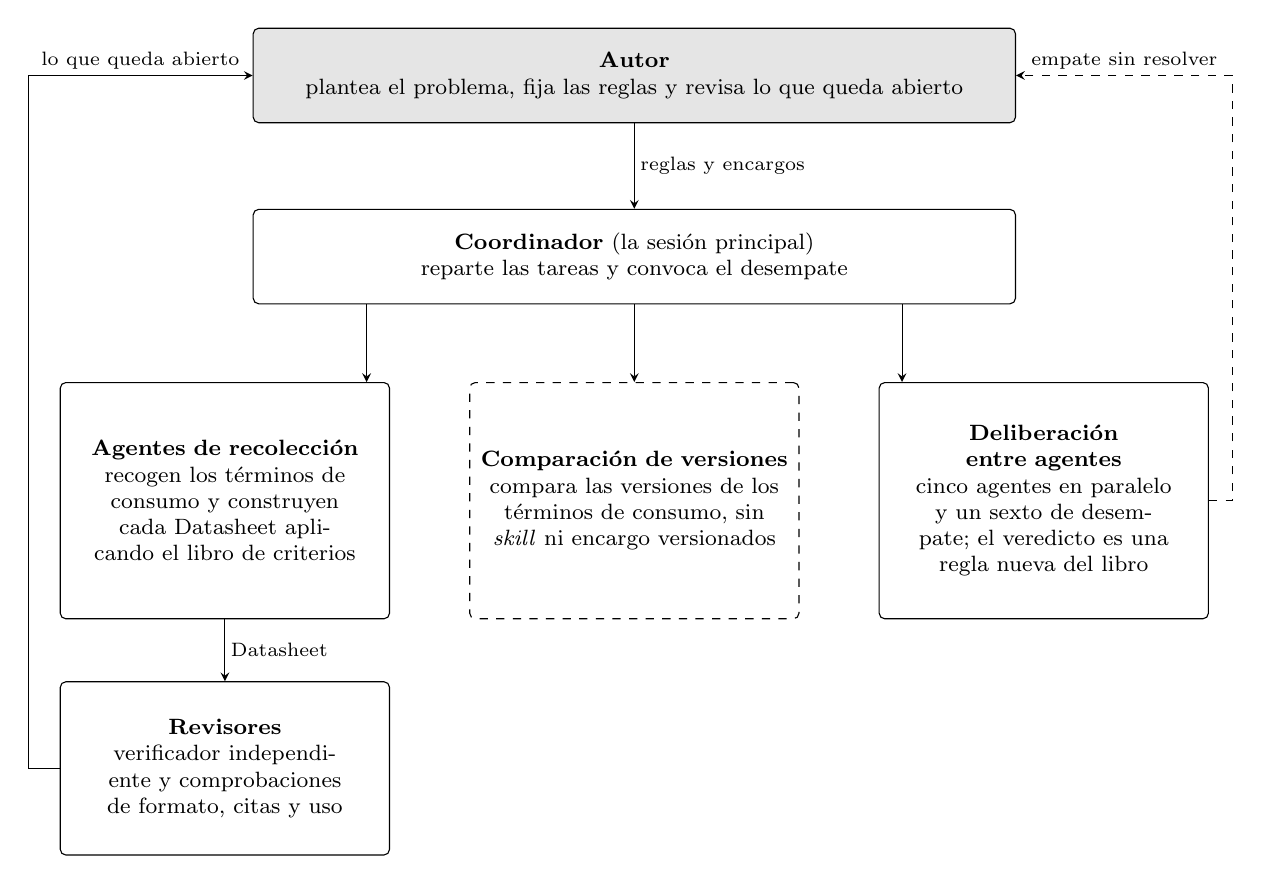
\begin{tikzpicture}[
  font=\footnotesize,
  caja/.style={draw, rounded corners=2pt, align=center, text width=3.9cm, minimum height=3cm, inner sep=4pt},
  ancha/.style={draw, rounded corners=2pt, align=center, text width=9.4cm, minimum height=1.2cm, inner sep=4pt},
  sinver/.style={dashed},
  etq/.style={font=\scriptsize, inner sep=2pt}
]
\node[ancha, fill=gray!20] (autor) at (7.9,0) {\textbf{Autor}\\ plantea el problema, fija las reglas y revisa lo que queda abierto};
\node[ancha] (coord) at (7.9,-2.3) {\textbf{Coordinador} (la sesión principal)\\ reparte las tareas y convoca el desempate};
\node[caja] (recol) at (2.7,-5.4) {\textbf{Agentes de recolección}\\ recogen los términos de consumo y construyen cada Datasheet aplicando el libro de criterios};
\node[caja, sinver] (diff) at (7.9,-5.4) {\textbf{Comparación de versiones}\\ compara las versiones de los términos de consumo, sin \textit{skill} ni encargo versionados};
\node[caja] (cons) at (13.1,-5.4) {\textbf{Deliberación entre agentes}\\ cinco agentes en paralelo y un sexto de desempate; el veredicto es una regla nueva del libro};
\node[caja, minimum height=2.2cm] (rev) at (2.7,-8.8) {\textbf{Revisores}\\ verificador independiente y comprobaciones de formato, citas y uso};
\draw[-stealth] (autor) -- node[etq, right] {reglas y encargos} (coord);
\draw[-stealth] (coord.south) ++(-3.4,0) coordinate (c1) -- (c1 |- recol.north);
\draw[-stealth] (coord.south) -- (diff.north);
\draw[-stealth] (coord.south) ++(3.4,0) coordinate (c3) -- (c3 |- cons.north);
\draw[-stealth] (recol) -- node[etq, right] {Datasheet} (rev);
\draw (rev.west) -- ++(-0.4,0) coordinate (a) -- (a |- autor);
\draw[-stealth] (a |- autor) -- node[etq, above] {lo que queda abierto} (autor.west);
\draw[dashed] (cons.east) -- ++(0.3,0) coordinate (b) -- (b |- autor);
\draw[-stealth, dashed] (b |- autor) -- node[etq, above] {empate sin resolver} (autor.east);
\end{tikzpicture}
\endgroup
\caption[Arquitectura de agentes del trabajo]{Arquitectura de agentes del trabajo. Las cajas de borde continuo son procesos documentados en el repositorio, y la de borde discontinuo, uno cuyo encargo y herramientas no están versionados. La flecha discontinua es el empate que la deliberación no resuelve.}
\label{fig:uso-ia:agentes}
\end{figure}

\section{Alcance del uso}

El trabajo se ha hecho con Claude, de Anthropic, en sus entornos Cowork y Claude Code, con la suscripción que imputa la Sección~\ref{sec:metodologia:presupuesto}.
Además de las dos consultas de las secciones siguientes y de la comparación entre versiones de los términos de consumo, Claude interviene en seis tareas.

\begin{description}
  \item[Construcción y revisión de las Datasheets.] Siguen el reparto de la Figura~\ref{fig:uso-ia:agentes}, salvo en la Datasheet de Postmark, que es anterior a él.
  \item[Recogida de los términos de consumo.] Una \textit{skill} propia, con validador y pruebas automáticas, captura en bruto las páginas de términos de consumo de cada proveedor (Sección~\ref{sec:propuesta:ciclo}).
  \item[Sondeos empíricos.] Las pruebas contra la API de un proveedor que miden un límite que su documentación no publica las ejecutan agentes, con un presupuesto declarado y con envíos limitados a tres direcciones del autor.
  \item[Análisis.] Los agentes preparan el recuento de en cuántas APIs reaparece cada elemento no soportado y las ejecuciones sobre PRIME4API, y sus resultados están versionados en el repositorio de datos.
  \item[Herramientas.] Los programas del repositorio, como el validador de formato o la verificación de citas, se programaron con Claude y tienen pruebas automáticas.
  \item[Redacción.] Claude ayuda en la redacción: propone versiones de los párrafos con el registro del autor, tomado de su Trabajo Fin de Grado, y las pasa por una \textit{skill} que quita las marcas de estilo habituales de los modelos de lenguaje. Otro agente, distinto del que las propone, comprueba que cada afirmación lleve su fuente y que el texto se entienda sin leer las referencias. El autor lee el texto completo, lo corrige y decide cada cambio.
\end{description}

Claude fue también objeto de una prueba, con las Datasheets en el prompt y sin ellas, sobre las cuatro preguntas del catálogo reservadas a HARVEY4API, el agente conversacional que consulta PRIME4API (Sección~\ref{sec:comparacion:harvey}).
La prueba no sustituye a HARVEY4API, que no se ejecutó en este trabajo: en ella el modelo hace él mismo las cuentas, sin llamar al motor.

\section{La consulta de la selección}

La selección de APIs del catálogo se completó con una consulta a un modelo de lenguaje (Sección~\ref{sec:propuesta:seleccion}).
El prompt pedía cuatro APIs seleccionadas y cuatro de reserva, ordenadas, con el tipo de modelo de precios de cada una y sin ninguna cifra.
La respuesta propuso Amazon SES, Brevo, Mailchimp Transactional y Mailgun, y de reserva, por este orden, Mailjet, Zoho ZeptoMail, SparkPost y SMTP2GO.
La Tabla~\ref{tab:uso-ia:ficha} recoge las condiciones de la consulta que constan en el fichero de la selección del repositorio, y también las que no constan.
El prompt literal y la respuesta íntegra están en el repositorio del trabajo\footnote{\url{https://github.com/danvelcam/tfm-pricing-apis-correo}, fichero \texttt{03\_datos/SELECCION\_APIS\_2026-09-01.md}. Contiene el prompt, la respuesta con su tabla de cobertura y la lista de reserva en su orden.}.

\begin{table}[H]
\centering
\small
\begin{tabular}{|p{4.2cm}|p{9.4cm}|}
\hline
\raggedright \textbf{Campo} & \raggedright \textbf{Valor} \tabularnewline
\hline
\raggedright Fecha & \raggedright 1 de septiembre de 2026 \tabularnewline
\hline
\raggedright Modelo & \raggedright \texttt{claude-fable-5-1}, de Anthropic \tabularnewline
\hline
\raggedright Entorno & \raggedright La sesión de trabajo del proyecto, a petición del autor \tabularnewline
\hline
\raggedright Criterios & \raggedright Cinco, ordenados por peso e incluidos en el prompt: diversidad del modelo de precios, documentación pública de precios y de límites, adopción en producción, un rasgo diferenciador de los límites y diversidad geográfica y de tamaño del proveedor \tabularnewline
\hline
\raggedright Catálogo previo & \raggedright Postmark, Resend, SendGrid y MailerSend, que el prompt excluye \tabularnewline
\hline
\raggedright Respuesta pedida & \raggedright Cuatro APIs seleccionadas y cuatro de reserva, ordenadas, y para cada una el tipo de modelo de precios, lo que aporta y el riesgo principal, sin inventar cifras \tabularnewline
\hline
\raggedright No consta en el fichero & \raggedright La hora, el prompt de sistema, los parámetros de generación, el número de intentos y la transcripción de la sesión \tabularnewline
\hline
\end{tabular}
\caption{Ficha de la consulta, según el fichero de la selección.}
\label{tab:uso-ia:ficha}
\end{table}

La consulta se hizo en la sesión de trabajo del proyecto, y la respuesta usa ese contexto: menciona dos decisiones de modelado anteriores que el prompt no recoge.
Una limita la Datasheet de Resend a su API de correo transaccional.
La otra pone \texttt{api\_first}, y no \texttt{partial\_saas}, en el campo \texttt{type} de un proveedor que tiene panel web y API.
Es el campo con el que ACM2YAML clasifica el servicio.
Este trabajo reserva \texttt{partial\_saas} para el servicio en el que alguna de tres operaciones (enviar, crear o editar una plantilla y añadir un dominio de envío) se puede hacer en el panel y no en la API, y en los demás casos usa \texttt{api\_first}.

\section{Cómo se aplicó}

La selección no cambió después de la consulta: ninguna API de la reserva sustituyó a una del catálogo (Apartado~\ref{sec:propuesta:reserva}).
La respuesta no da precios ni límites con cifra, así que ninguno de los que recoge el catálogo procede de ella.
Cada uno sale de la documentación del proveedor, de su panel o de un sondeo, en la ventana de toma de datos (Apartado~\ref{sec:propuesta:ventana}).
La construcción corrigió tres afirmaciones de la respuesta, sobre Amazon SES, Mailgun y Brevo, y la Sección~\ref{sec:propuesta:respuesta} las detalla.

Una segunda consulta, ajena a la selección, preguntó a Claude Opus 5.5 si doce elementos no soportados que aparecen en una sola API admiten una forma general que valga también para otros proveedores.
Once son los que el inventario no promueve al modelo.
El duodécimo era un supuesto tercer tope diario de MailerSend, de 100 correos en el plan Free, sin sitio en la Datasheet porque el plan y el \textit{endpoint} ya tenían cada uno su cuota.
Se retiró dos días después de la consulta: la página de precios cifra ese tope en peticiones, y en peticiones es la cuota diaria que la Datasheet ya tenía.
La respuesta a esa consulta no cambia ningún dato del catálogo ni el veredicto de ningún elemento (Sección~\ref{sec:propuesta:conformidad}).
